

\tikzset{every picture/.style={line width=0.75pt}} %set default line width to 0.75pt        

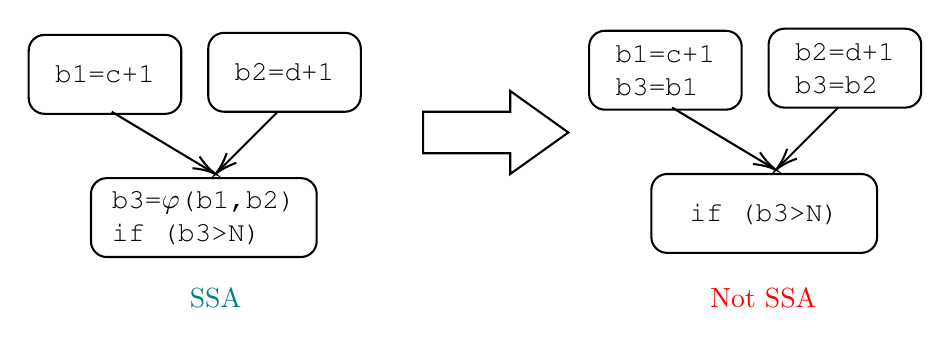
\begin{tikzpicture}[x=0.75pt,y=0.75pt,yscale=-1,xscale=1]
%uncomment if require: \path (0,139.6999969482422); %set diagram left start at 0, and has height of 139.6999969482422

%Rounded Rect [id:dp262243382651531] 
\draw   (10,20.6) .. controls (10,16.4) and (13.4,13) .. (17.6,13) -- (75.9,13) .. controls (80.1,13) and (83.5,16.4) .. (83.5,20.6) -- (83.5,43.4) .. controls (83.5,47.6) and (80.1,51) .. (75.9,51) -- (17.6,51) .. controls (13.4,51) and (10,47.6) .. (10,43.4) -- cycle ;
%Rounded Rect [id:dp4192314773958711] 
\draw   (96.5,19.6) .. controls (96.5,15.4) and (99.9,12) .. (104.1,12) -- (162.4,12) .. controls (166.6,12) and (170,15.4) .. (170,19.6) -- (170,42.4) .. controls (170,46.6) and (166.6,50) .. (162.4,50) -- (104.1,50) .. controls (99.9,50) and (96.5,46.6) .. (96.5,42.4) -- cycle ;
%Rounded Rect [id:dp14874696406611254] 
\draw   (40,89.6) .. controls (40,85.4) and (43.4,82) .. (47.6,82) -- (141.15,82) .. controls (145.35,82) and (148.75,85.4) .. (148.75,89.6) -- (148.75,112.4) .. controls (148.75,116.6) and (145.35,120) .. (141.15,120) -- (47.6,120) .. controls (43.4,120) and (40,116.6) .. (40,112.4) -- cycle ;
%Straight Lines [id:da8036054523449865] 
\draw    (50,50) -- (98.29,78.97) ;
\draw [shift={(100,80)}, rotate = 210.96] [color={rgb, 255:red, 0; green, 0; blue, 0 }  ][line width=0.75]    (10.93,-3.29) .. controls (6.95,-1.4) and (3.31,-0.3) .. (0,0) .. controls (3.31,0.3) and (6.95,1.4) .. (10.93,3.29)   ;

%Straight Lines [id:da9462543361304327] 
\draw    (130,50) -- (101.41,78.59) ;
\draw [shift={(100,80)}, rotate = 315] [color={rgb, 255:red, 0; green, 0; blue, 0 }  ][line width=0.75]    (10.93,-3.29) .. controls (6.95,-1.4) and (3.31,-0.3) .. (0,0) .. controls (3.31,0.3) and (6.95,1.4) .. (10.93,3.29)   ;

%Right Arrow [id:dp5454010361665674] 
\draw   (200,50) -- (242,50) -- (242,40) -- (270,60) -- (242,80) -- (242,70) -- (200,70) -- cycle ;
%Rounded Rect [id:dp804370127764321] 
\draw   (280,18.6) .. controls (280,14.4) and (283.4,11) .. (287.6,11) -- (345.9,11) .. controls (350.1,11) and (353.5,14.4) .. (353.5,18.6) -- (353.5,41.4) .. controls (353.5,45.6) and (350.1,49) .. (345.9,49) -- (287.6,49) .. controls (283.4,49) and (280,45.6) .. (280,41.4) -- cycle ;
%Rounded Rect [id:dp054537017000311994] 
\draw   (366.5,17.6) .. controls (366.5,13.4) and (369.9,10) .. (374.1,10) -- (432.4,10) .. controls (436.6,10) and (440,13.4) .. (440,17.6) -- (440,40.4) .. controls (440,44.6) and (436.6,48) .. (432.4,48) -- (374.1,48) .. controls (369.9,48) and (366.5,44.6) .. (366.5,40.4) -- cycle ;
%Rounded Rect [id:dp9347541053691467] 
\draw   (310,87.6) .. controls (310,83.4) and (313.4,80) .. (317.6,80) -- (411.15,80) .. controls (415.35,80) and (418.75,83.4) .. (418.75,87.6) -- (418.75,110.4) .. controls (418.75,114.6) and (415.35,118) .. (411.15,118) -- (317.6,118) .. controls (313.4,118) and (310,114.6) .. (310,110.4) -- cycle ;
%Straight Lines [id:da09161146890023963] 
\draw    (320,48) -- (368.29,76.97) ;
\draw [shift={(370,78)}, rotate = 210.96] [color={rgb, 255:red, 0; green, 0; blue, 0 }  ][line width=0.75]    (10.93,-3.29) .. controls (6.95,-1.4) and (3.31,-0.3) .. (0,0) .. controls (3.31,0.3) and (6.95,1.4) .. (10.93,3.29)   ;

%Straight Lines [id:da9445970974561072] 
\draw    (400,48) -- (371.41,76.59) ;
\draw [shift={(370,78)}, rotate = 315] [color={rgb, 255:red, 0; green, 0; blue, 0 }  ][line width=0.75]    (10.93,-3.29) .. controls (6.95,-1.4) and (3.31,-0.3) .. (0,0) .. controls (3.31,0.3) and (6.95,1.4) .. (10.93,3.29)   ;


% Text Node
\draw (46.75,32) node  [align=left] {{\fontfamily{pcr}\selectfont b1=c+1}};
% Text Node
\draw (133.25,31) node  [align=left] {{\fontfamily{pcr}\selectfont b2=d+1}};
% Text Node
\draw (94.38,101) node  [align=left] {{\fontfamily{pcr}\selectfont b3=$\varphi$(b1,b2)}\\{\fontfamily{pcr}\selectfont if (b3>N)}};
% Text Node
\draw (316.75,30) node  [align=left] {{\fontfamily{pcr}\selectfont b1=c+1}\\{\fontfamily{pcr}\selectfont b3=b1}};
% Text Node
\draw (403.25,29) node  [align=left] {{\fontfamily{pcr}\selectfont b2=d+1}\\{\fontfamily{pcr}\selectfont b3=b2}};
% Text Node
\draw (364.38,99) node  [align=left] {{\fontfamily{pcr}\selectfont if (b3>N)}};

\draw (100,140) node  [align=left] {\textcolor{teal}{SSA}};
\draw (364,140) node  [align=left] {\textcolor{red}{Not SSA}};


\end{tikzpicture}
